\documentclass[hidelinks,11pt,dvipsnames]{article}
% xcolor commonly causes option clashes, this fixes that
\PassOptionsToPackage{dvipsnames,table}{xcolor}
\usepackage[tmargin=1in, bmargin=1in, lmargin=0.8in, rmargin=1in]{geometry}

%%%%%%%%%%%%%%%%%%%%%%%%%%%%%%%%%%%%%%%%%%%%%%%%%%%%%%%%%%%%%%%%%%%%
%%% For inkscape-figures
%%% Assumes the following directory structure:
%%% master.tex
%%% figures/
%%%     figure1.pdf_tex
%%%     figure1.svg
%%%     figure1.pdf
%%%%%%%%%%%%%%%%%%%%%%%%%%%%%%%%%%%%%%%%%%%%%%%%%%%%%%%%%%%%%%%%%%%%
%\usepackage{import}
\usepackage{pdfpages}
\usepackage{transparent}

\newcommand{\incfig}[2][1]{%
    \def\svgwidth{#1\columnwidth}
    \import{./figures/}{#2.pdf_tex}
}

\pdfsuppresswarningpagegroup=1

% enable synctex for inverse search, whatever synctex is
\synctex=1
\usepackage{float,macrosabound,homework,theorem-env}
\usepackage{microtype}


% font stuff
\usepackage{sectsty}
\allsectionsfont{\sffamily}
\linespread{1.1}

% bibtex stuff
\usepackage[backend=biber,style=alphabetic,sorting=anyt]{biblatex}
\addbibresource{main.bib}

% colored text shortcuts
\newcommand{\blue}[1]{\color{MidnightBlue}{#1}}
\newcommand{\red}[1]{\textcolor{Mahogany}{#1}}
\newcommand{\green}[1]{\textcolor{ForestGreen}{#1}}


% use mathptmx pkg while using default mathcal font
\DeclareMathAlphabet{\mathcal}{OMS}{cmsy}{m}{n}

% fixes the positioning of subscripts in $$ $$
\renewcommand{\det}{\operatorname{det}}

\usetikzlibrary{positioning, arrows.meta}
\newcommand{\here}[2]{\tikz[remember picture]{\node[inner sep=0](#2){#1}}}

%%%%%%%%%%%%%%%%%%%%%%%%%%%%%%%%%%%%%%%%%%%%%%%%%%%%%%%%%%%%%%%%%%%%%
%%% Entry Counter
%%%%%%%%%%%%%%%%%%%%%%%%%%%%%%%%%%%%%%%%%%%%%%%%%%%%%%%%%%%%%%%%%%%%%
\newcounter{entry-counter}
\newcommand{\entry}[1]
{
	\addtocounter{entry-counter}{1}
    \tchap{Entry \arabic{entry-counter}}
	%\addcontentsline{toc}{section}{Entry \arabic{entry-counter}: #1}
	\vspace{-1.5em}
    \begin{center}
		\small \emph{Written: #1}
    \end{center}
}

\usepackage{titling}
\renewcommand\maketitlehooka{\null\mbox{}\vfill}
\renewcommand\maketitlehookd{\vfill\null}


\usepackage{capt-of}
\usepackage{tikz}
\usetikzlibrary{positioning,calc,intersections,through,backgrounds, shapes.geometric, decorations.markings,arrows}

\def\sset{\subseteq}
\def\iso{\cong}
\def\gend#1{\langle #1\rangle}

\newcommand{\rightoverleftarrow}{%
  \mathrel{\vcenter{\mathsurround0pt
    \ialign{##\crcr
      \noalign{\nointerlineskip}$\longrightarrow$\crcr
      \noalign{\nointerlineskip}$\longleftarrow$\crcr
    }%
  }}%
}

\newcommand\makesphere{} % just for safety
\def\makesphere(#1)(#2)[#3][#4]{%
  % Synopsis
  % \makesphere[draw options](center)(initial angle:final angle:radius)
  \shade[ball color = #3, opacity = #4] #1 circle (#2);
  \draw #1 circle (#2);
  \draw ($#1 - (#2, 0)$) arc (180:360:#2 and 3*#2/10);
  \draw[dashed] ($#1 + (#2, 0)$) arc (0:180:#2 and 3*#2/10);
}
% same thing as makesphere but places white background behind
\newcommand\altmakesphere{} % just for safety
\def\altmakesphere(#1)(#2)(#3)[#4][#5]{%
  % Synopsis
  % \make sphere[draw options](center)(initial angle:final angle:radius)
  \draw [fill=white!30] #1 circle (#2);
  \shade[ball color = #4, opacity = #5] #1 circle (#2);
  \draw #1 circle (#2);
  \draw ($#1 - (#2, 0)$) arc (180:360:#2 and 3*#2/10);
  \draw[dashed] ($#1 + (#2, 0)$) arc (0:180:#2 and 3*#2/10);
  \node at #1 {#3};
}

\begin{document}
% set section number to 1
% fixes theorem numbering without need to have a section title
\setcounter{section}{1}

\pagestyle{empty}
	\LARGE
\begin{center}
	Algebraic Topology Homework 9 \\
	\Large
	Isaac Martin \\
    Last compiled \today
\end{center}
\normalsize
\vspace{-4mm}
\hru

\tchap{Problems from 2.1}

\begin{homework}[e]
  \prob[\textsc{Exercise }2.1.20] Show that $\tilH_n(X) \approx \tilH_{n+1}(SX)$ for all $n$, where $SX$ is the suspension of $X$. More generally, thinking of $SX$ as the union of two cones $CX$ with their bases identified, compute the reduced homology groups of the union of any finite number of cones $CX$ with their bases identified.
  \begin{prf}
    The suspension $SX$ of $X$ is the disjoint union of two cones of $X$ with bases identified. For instance, the suspension of $S^n$ is $S^{n+1}$, so this proof will likely bear resemblance to the calculation of $H_i(S^n)$. Write $SX = C_1X\cup C_2X$ where $C_1X$ and $C_2X$ are the two cones in question, with the understanding that their bases are identified. The inclusion $C_2X \hookrightarrow SX$ induces a chain of short exact sequences whose rows are given by
    \begin{align*}
      0 \to C_n(C_2X) \to C_n(SX) \to C_n(SX,C_2X) \to 0,
    \end{align*}
    and because $C_2(X)$ is contractible, $H_n(C_2X) \cong 0$ for all $n \geq 1$. This means the long exact sequence in homology induced by these short exact sequences of chains is
    \begin{align*}
      ... \to 0 \to \tilH_n(SX) \to H_n(SX,C_2X) \to 0 \to ...
    \end{align*}
    away from $n = 0$, so we have isomorphisms $\tilH_n(SX) \cong \tilH_n(SX,C_2X)$ whenever $n \geq 1$. Because $SX$ is path connected through the tips of its cones, this isomorphism holds at $n = 0$ as well, where all the homology groups in question are simply $\bZ$ and hence the reduced homology groups are all trivial.

    Now notice that $C_1X$ and $C_2X$ share a base homeomorphic to $X$, so $C_1X\cap C_2X = X$. Applying the excision theorem (the version which looks at the inclusion $(B,B\cap A)\hookrightarrow (X,A)$) to the pairs $(C_1X,X) \hookrightarrow (SX,C_2X)$ induces an isomorphism $\tilH_n(C_1X,X) \cong \tilH_n(SX,C_2X) \cong \tilH_n(SX)$ for all $n$. Technically, we actually need to take slightly enlarged copies of $C_1X$ and $C_2X$, since we require the \emph{interiors} of $C_1X$ and $C_2X$ cover $SX$ for the excision theorem to apply. However, these enlarged copies can be chosen in such a way so that they deformation retract to $C_1X$ and $C_2X$ meaning that morally we are okay to ignore this detail. To get the desired isomorphism, we simply look at the long exact sequence of the pair $(C_1X,X)$ which reads
    \begin{align*}
      ... \to \tilH_{n+1}(C_1X) \to \tilH_{n+1}(C_1X,X) \to \tilH_n(X) \to \tilH_n(C_1X) \to ...
    \end{align*}
    Because $C_1X$ is contractible, $\tilH_n(C_1X) \cong 0$ for all $n$, and hence we have isomorphisms $\tilH_n(X) \cong \tilH_{n+1}(C_1X,X) \cong \tilH_{n+1}(SX)$.

    \bigskip

    The above argument relied on the fact that $C_1X$ and $C_2X$ were contractible and were glued along a base homeomorphic to $X$, so if we attach more copies of the cone of $X$ to the same base, we ought to get a similar result. Let $S_kX$ denote the ``suspension of $X$'' with $k$ copies of $CX$ attached to $X$. It's clear that $S_{k+1}X = S_kX \cup CX$, so we proceed inductively. Repeating the argument above with $S_kX$ in the place of $C_1X$ and $CX$ in the place of $C_2X$, everything works up until we make use of the con tractability of $C_1X$. Indeed, $S_kX$ need not be contractible. This does get us to the following point, however:
    \begin{align*}
      \tilH_{n+1}(S_{k+1}X) \cong \tilH_{n+1}(S_kX,X).
    \end{align*}
    However, $CX / X \simeq SX$, where $X$ is understood to be the base of $CX$. This is easy to see from the construction of $CX$: it is $X\times I / X\times \{1\}$. The suspension $SX$ is obtained by identifying two copies of $CX$ at the base, or equivalently, $SX \cong X\times I / (X\times \{1\} \cup X\times \{0\})$.
    \begin{center}
      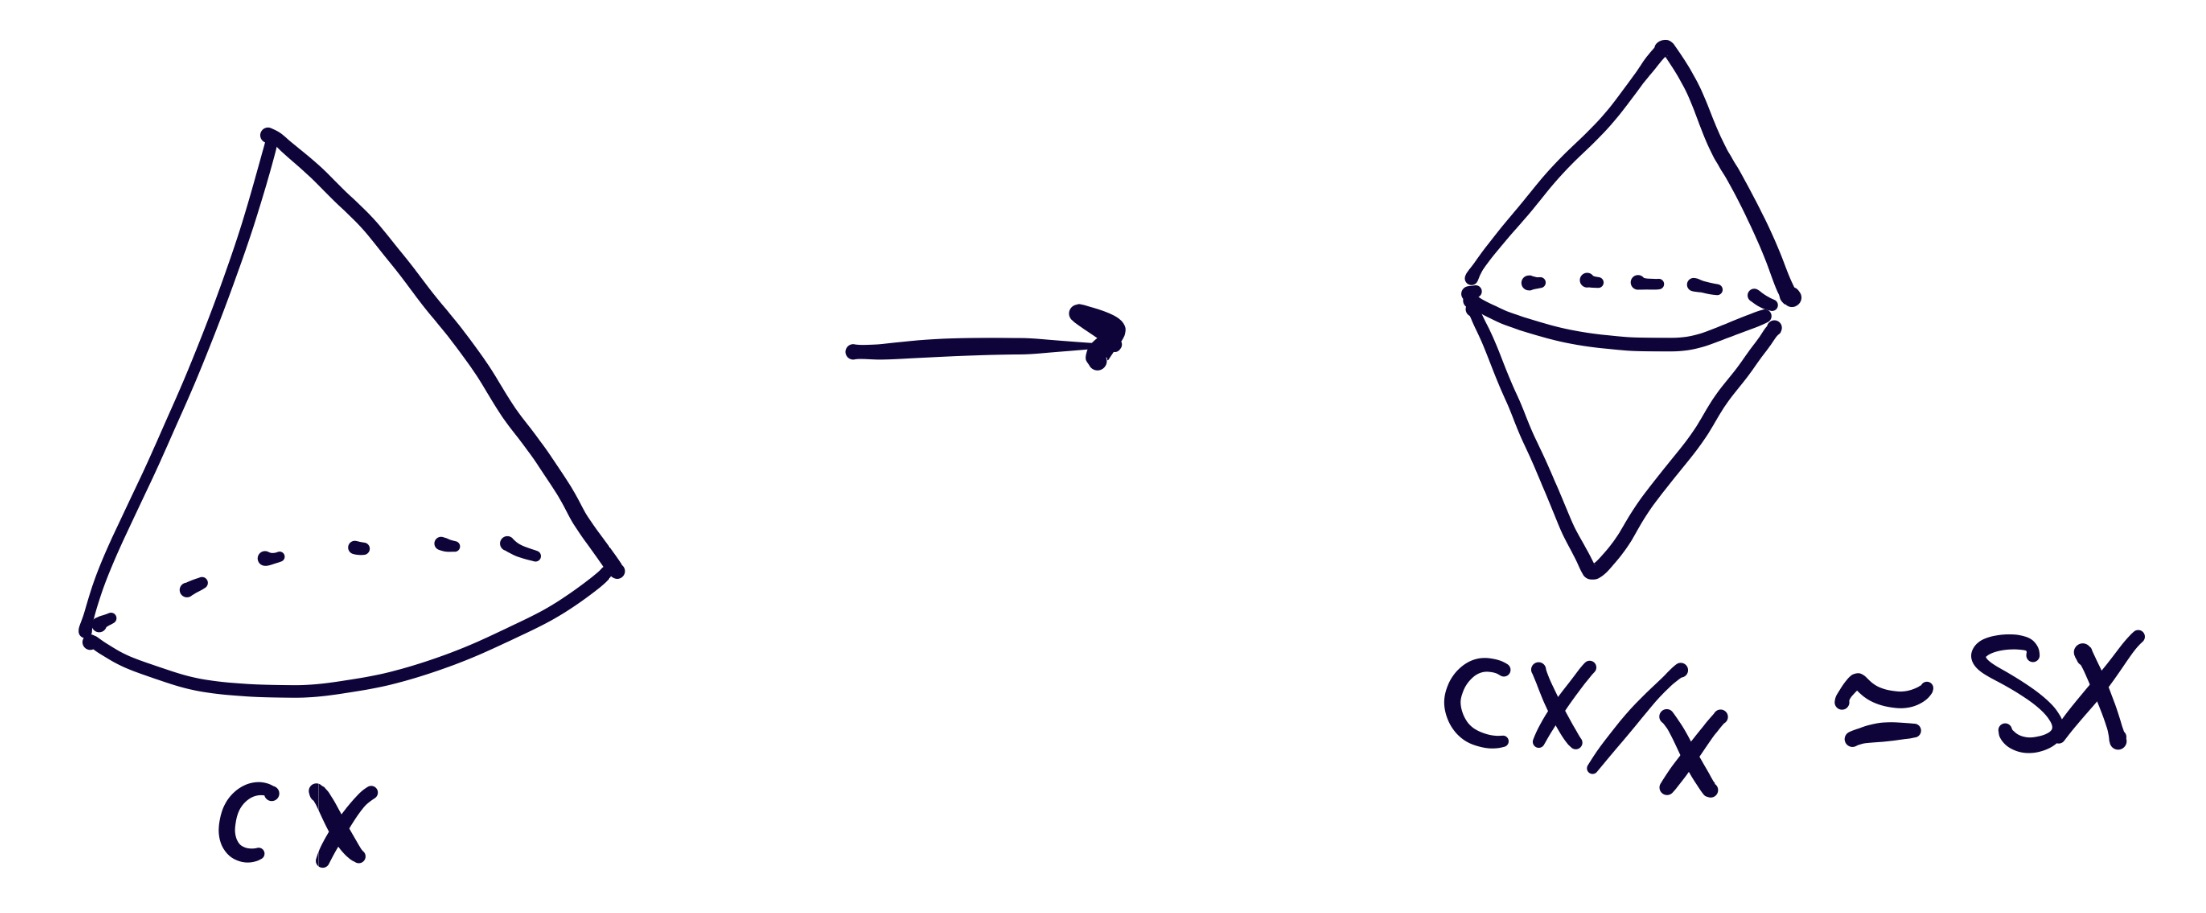
\includegraphics[width=12cm]{figures/hwk9-fig1.png}
      \captionof{figure}{Collapsing the base of a cone to a point produces $SX$}
      \label{fig:prob1-1}
    \end{center}
    Now consider what happens when we collapse the common base of the cones comprising $S_{k}X$. Each copy of $CX$ becomes a copy of $SX$, and each $SX$ meets every other $SX$ at the newly formed point resulting from the quotient by $X$.
    \begin{center}
      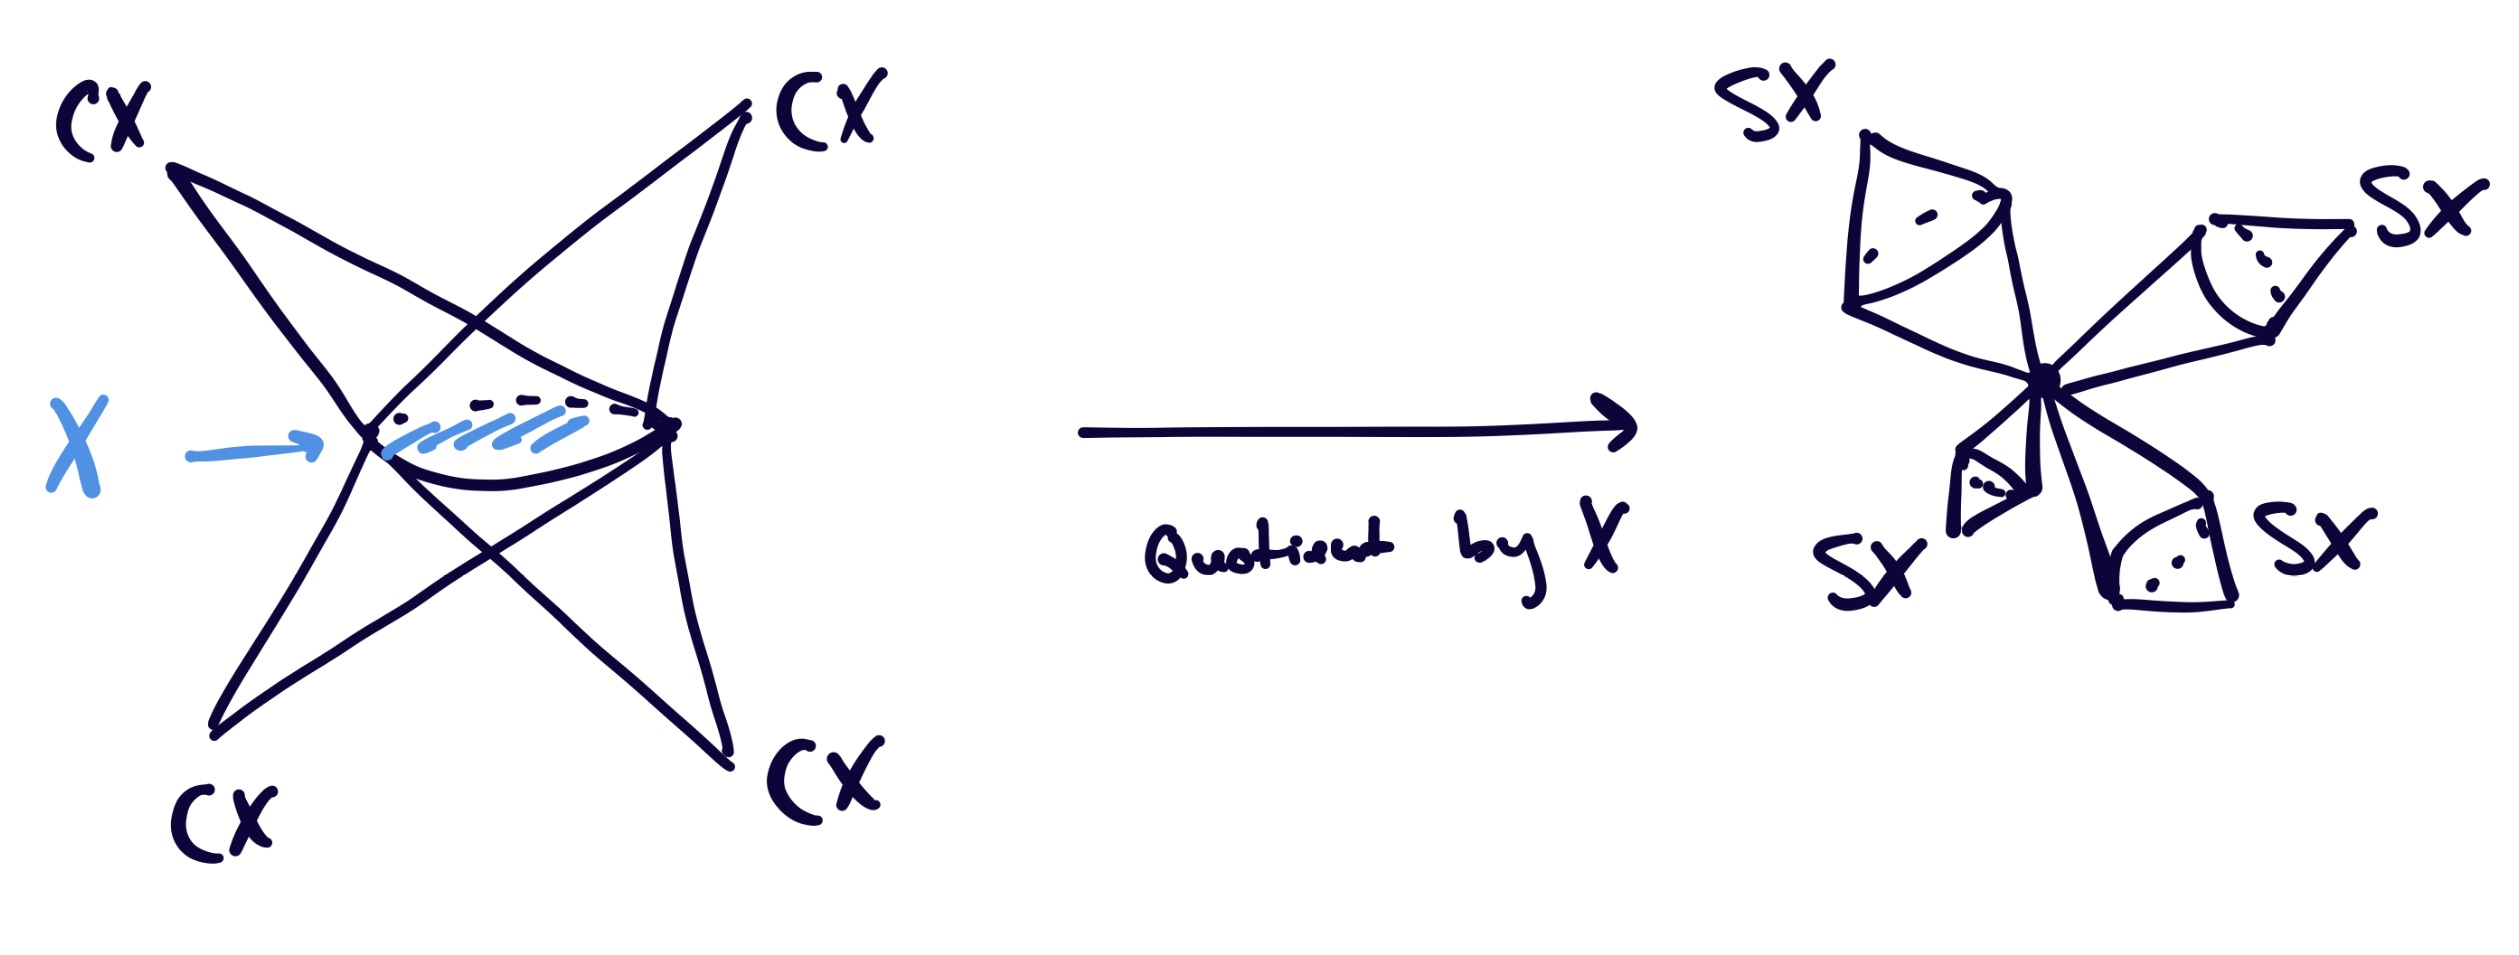
\includegraphics[width=12cm]{figures/hwk9-fig2.png}
      \captionof{figure}{Collapsing the common base of $C_1X \cup C_2X \cup...\cup C_kX$ to a point produces $SX\vee SX \vee...\vee SX$.}
      \label{fig:prob1-2}
    \end{center}
    Hence,
    \begin{align*}
      \tilH_{n+1}(S_kX,X) \cong \tilH_{n+1}(S_kX/X) \cong \tilH_{n+1}(SX\vee...\vee SX) \cong \bigoplus_{i=1}^k H_{n+1}(SX) \cong \bigoplus^k_{i=1} \tilH_n(X)
    \end{align*}
    for all $n$, where we have used the fact $\tilH_n(X) \cong \tilH_{n+1}(SX)$.
  \end{prf}
  \prob[\textsc{Exercise }2.1.21] Making the preceding problem more concrete, construct explicit chain maps $s:C_n(X) \to C_{n+1}(SX)$ inducing isomorphisms $\tilH_n(X) \to \tilH_{n+1}(SX)$.
  \begin{prf}
    Consider the following maps of chain complexes:
    \begin{align*}
      C_n(X) \xrightarrow{\alpha} C_{n+1}(CX,X) \xrightarrow{\beta} C_{n+1}(SX).
    \end{align*}
    We previously showed that $\tilH_n(X) \cong \tilH_{n+1}(CX,X)\cong \tilH_{n+1}(SX)$, so this seems like a good sequence to consider. How are these chain maps defined? The map $\alpha$ takes a singular simplex $\sigma:\Delta^n\to X$ to $C\sigma:C\Delta^n\to CX$. However, the cone of any $n$-simplex is an $n+1$-simplex, so $C\Delta^n\to CX$ can instead be considered as a mapping $\Delta^{n+1}\to CX$. The map $C\sigma$ can be written down explicitly: given any point $(t_0,...,t_{n+1})\in \Delta^{n+1} = C\Delta^{n}$,
    \begin{align*}
      C\sigma(t_0,...,t_{n+1}) = \sum_{i=1}^n t_i\sigma(v_i) + t_{n+1}p
    \end{align*}
    where $p \in CX$ is the cone point, i.e. the point resulting from collapsing $X\times \{1\}$. $C\sigma$ first takes the simplex $\sigma$ into the copy of $X$ comprising the base of $CX$ and then takes the cone.

    Anyways, removing $v_i$ from the simplex $[v_0,...,v_{n+1}]$ is equivalent to setting $t_i = 0$, so from the definition of $C\sigma$ we immediately get
    \begin{align*}
      (C\sigma)|_{[v_0,...,\hatv_i,...,v_{n+1}]} = C(\sigma|_{[v_0,...,\hatv_i,...,v_{n+1}]})
    \end{align*}
    whenever $0\leq i\leq n$ and
    \begin{align*}
      (C\sigma)|_{[v_0,...,v_n,\hatv_{n+1}]} = \sigma
    \end{align*}
    for $i = n+1$, where $\sigma$ here is interpreted as the original map $\sigma:\Delta^n\to X$ composed with the homeomorphism $X \to X\times \{1\}\subseteq CX$. We can now compute $\partial (C\sigma)$:
    \begin{align*}
      \partial(C\sigma) &~=~ \sum_{i=0}^{n+1}(-1)^i(C\sigma)|_{[v_0,...,\hatv_i,...,v_{n+1}]} \\
                        &~=~\sum_{i=0}^{n} (-1)^iC(\sigma|_{[v_0,...,\hatv_i,...,v_{n+1}]}) + (-1)^{n+1}\sigma \\
                        &~=~ C(\partial \sigma) + (-1)^{n+1}\sigma.
    \end{align*}
    We used the linearity of $C$ on chains to move the sum inside the argument of $C$. A small neighborhood $X \times [0,\epsilon)$ of $X\times \{0\}$ inside $CX$ deformation retracts to $X\times \{0\}$, so the pair $(CX,X)$ is a good pair (where $X$ is identified with $X\times \{0\}$, as usual) and gives us the following long exact sequence on homology:
    \begin{align*}
      ...\to \tilH_{n+1}(CX) \to \tilH_{n+1}(CX,X) \xrightarrow{\partial}\tilH_{n}(X) \to \tilH_n(CX) \to ...
    \end{align*}
    which gives us isomorphisms $\partial:\tilH_{n+1}(CX,X) \xrightarrow{\sim} \tilH_n(X)$ since $CX$ is contractible and hence $\tilH_n(CX) = 0$. 

    Now consider the linear extension $f$ of $\alpha$, the map taking $\sigma\mapsto C\sigma$ above. We show that $f_*\partial$ is the identity on $\tilH_{n+1}(CX,X)$. Given a relative cycle $\gamma \in C_{n+1}(CX,X)$ the boundary $\partial \gamma$ lies in $C_n(X)$. However, $f_*[\partial(\gamma)] = [f_*(\partial\gamma)]$, and $f$ acts on $\partial\gamma$ by extending it to a cone. This means $f$ precisely ``undoes'' the action of $\partial$, so
    \begin{align*}
      f_*\partial[\gamma] = f_*[\partial \gamma] = [\gamma].
    \end{align*}
    Since $f_*\partial$  is the identity and $\partial$ is an isomorphism, $f_*$ must also be an isomorphism.

    Now, because $(CX,X)$ is a good pair, the quotient $q:(CX,X) \to (CX/X,X/X) \cong (SX,\text{pt})$ induces an isomorphism $q_*:\tilH_*(CX,X) \cong\tilH_*(SX,\text{pt})$. This gives us an isomorphism $q_*\circ f_*:\tilH_n(X) \to \tilH_{n+1}(SX,\text{pt}) \cong \tilH_{n+1}(SX)$ corresponding to the chain map $q\circ f$.
  \end{prf}
  \prob[\textsc{Exercise }2.1.23] Show that the second barycentric subdivision of a $\Delta$-complex is a simplicial complex. Namely, show that the first barycentric subdivision produces a $\Delta$-complex with the property that each simplex has all its vertices distinct, then show that for a $\Delta$-complex with this property, barycentric subdivision produces a simplicial complex.
  \begin{prf}
    I was stuck on this one for a while, I had to find a stack overflow post for the following hint (https://math.stackexchange.com/questions/1050085/a-question-about-hatcher-exercise-2-1-23). It suggested splitting this argument up into two parts: 
    \begin{enumerate}[(A)]
      \item We show that if $X$ is a $\Delta$-complex with $k$-skeleton $X^k$, then $B(X^k)$ is comprised of simplicies whose vertices are distinct.
      \item We show that if $X$ is a $\Delta$-complex such that each $k$-simplex has distinct vertices, then $B(X)$ is a simplicial complex.
    \end{enumerate}
    If both implications are true, then the second barycentric subdivision of an arbitrary $\Delta$-complex will be a simplicial complex.

    \bigskip

    \noindent \textbf{\emph{(A)}}\hspace{1em} We argue inductively on the dimension of $X$, the $\Delta$-complex.

    In the base case, $X$ is a $1$-simplex homeomorphic to an interval $[a,b]$. Barycentric subdivision gives us \emph{two} intervals $\left[a,\frac{a+b}{2}\right]$ and $\left[\frac{a+b}{2},b\right]$. These two $1$-simplicies have distinct vertices, $a$ and $b$.

    Now suppose that $(A)$ holds for all $k < n$, i.e. that if $X$ is a $\Delta$-complex then for all $k < n$ the $k$-simplicies of $B(X)$ are comprised of distinct vertices. For each $n$-simplex $X^n = [x_0,...,x_n]$ with barycenter $b$ in $X$, we get $n$ subsimplices $X_i^n = [b,x_0,...,\hatx_i,...,x_n]$. Passing to the boundary maps, we get that
    \begin{align*}
      \partial X^i_n = \sum_{j \neq i} (-1)^j[b,x_0,...,\hatx_j,...,x_n]
    \end{align*}
    noting that $x_i$ is omitted from $[b,x_0,...,\hatx_j,...,x_n]$. For $j\neq \ell$, $[b,x_0,...,\hatx_j,...,x_n]\neq [b,x_0,...,\hatx_\ell,...,x_n]$ by the inductive hypothesis. Since each $X^i$ omits a different vertex $x_i$, this shows that $X^n_i = X^n_{i'}$ if and only if $i = i'$, meaning that all the subsimplices have distinct vertices. Hence $B(X^n)$ is made up of $n$-simplicies whose vertices are all distinct from one another.

    \bigskip

    \noindent \textbf{\emph{(B)}}\hspace{1em} Now suppose that $X^n$ is the $n$-skeleton of a $\Delta$-complex $X$ whose $k$-simplicies are comprised of distinct vertices. We prove that $B(X^n)$ is a simplicial complex by induction.

    Consider $X^1$ for the base case. This is comprised solely of $1$-simplicies which we enumerate $X^1_i$ so that $\partial X^1_i = \{a_i,b_i\}$. Suppose two 1-simplicies have the same endpoints, i.e. if $a_i = a_j$ and $b_i = b_j$ for some $i$ and $j$. Once we barycentric subdivide we add two points $m_i$ and $m_j$ so that $B(X^1_i) \cong [a_i,m_i]\cup [m_i,b_i]$ and $B(X^1_j) = [a_j,m_j]\cup [m_j,b_j]$. By the inductive hypothesis, $a_i \neq m_i \neq b_i$, and because $X^1_i$ and $X^1_j$ are distinct, $m_i \neq m_j$. This means $B(X^1_i)$ has at least one vertex distinct from $B(X^1_j)$ for all $i \neq j$, and hence $B(X^1)$ is a simplicial complex.

    We now proceed to the inductive step. Suppose that $B(X^k)$ is a simplicial complex $\forall k < n$ and that $X^n_i = [x_0,...,x_n]$ and $X^n_j = [y_0,...,y_n]$ are two $n$-simplicies in $X^n$ which share the same vertices. The barycentric subdivision again introduces two barycenters $b_i$ and $b_j$ which are necessarily distinct whenever $i\neq j$ (since $X^n_i$ and $X^n_j$ are distinct).

    Using the same argument as in part (A), $\partial B(X^n_i)$ and $\partial B(X^n_j)$ are given by alternating sums of $n-1$ simplicies which are coned over $b_i$ and $b_j$ respectively. Since the barycenters aren't equal, each term of $\partial B(X^n_i)$ and $\partial B(X^n_j)$ are distinct. This means $B(X^n_i)$ And $B(X^n_j)$ have distinct vertices from one another whenever $i\neq j$.

    Therefore, $B(X)$ is a simplicial complex by induction, and by applying barycentric subdivision to an arbitrary $\Delta$-complex twice we obtain a simplicial complex.
  \end{prf}
  \prob[\textsc{Exercise }2.1.29] Show that $S^1\times S^1$ and $S^1 \vee S^1 \vee S^2$ have isomorphic homology groups in all dimensions, but their universal covering spaces do not.
  \begin{prf}
    We already know the homology groups of the torus:
    \begin{align*}
      H_n(S^1\times S^1) \cong
      \begin{cases}
        \bZ & n \in \{0,2\} \\
        \bZ^2 & n = 1 \\
        0 & else
      \end{cases},
    \end{align*}
    so we must now compute the homology of $S^1\vee S^1\vee S^2$. Corollary 2.25 seems handy for this situation, it says that the $n^{th}$ reduced horology of a wedge sum $\bigvee_\alpha X_\alpha A$ is isomorphic to $\bigoplus_\alpha \tilH_n(X_\alpha)$, provided that the basepoints $x_\alpha \in X_\alpha$ of the identifications are all good pairs. Luckily, for any point $x \in S^1$ or $y \in S^2$, the pairs $(S^1,x)$ and $(S^2,y)$ are good pairs. One way to see this is that we may take a small $\epsilon$-neighborhood of $x$ in $S^1$ homeomorphic to an interval or of $y$ in $S^2$ homeomorphic to an open disk, in either case, these neighborhoods deformation retract to $x$ and $y$ respectively. Hence, we can use Corollary 2.25 to calculate the homology of $S^1\vee S^1\vee S^2$ and get
    \begin{align*}
      \tilH_{n}(S^1\vee S^1 \vee S^1) \cong \tilH_n(S^1)^{\oplus 2} \oplus \tilH_n(S^2) \cong 
      \begin{cases}
        \bZ & n = 2 \\
        \bZ^{\oplus 2} & n = 1 \\
        0 & else
      \end{cases}
    \end{align*}
    from our knowledge of the homology of a sphere. Converting from reduced to ``typical'' homology gives us $H_0(S^1\vee S^1\vee S^2) \cong \bZ$, so the homology groups of $S^1\times S^1$ and $S^1\vee S^1\vee S^2$ do indeed match.

    \bigskip

    We now turn our attention to covering spaces. The torus $S^1\times S^1$ can be realized as the quotient $\bR^2/\bZ^2$, hence we have a quotient map $\pi:\bR^2 \to S^1\times S^1$. This is easily seen to be a covering map as each open square $(n,n+1)\times (m,m+1)\subseteq \bR^2$ maps homeomorphically to $S^1\times S^1 - (S^1\vee S^1)$. Since $\bR^2$ is simply connected, it is thus the universal cover of $S^1\times S^1$. The plane $\bR^2$ is contractible, and hence has only trivial reduced homology groups.

    Recall that we constructed the universal cover of $S^1\vee S^1\vee S^2$ in a previous exercise. It is obtained by attaching a copy of $S^2$ at every vertex of the universal cover of $S^1\vee S^1$, as seen in Figure (\ref{fig:prob4-1}).
    \begin{center}
      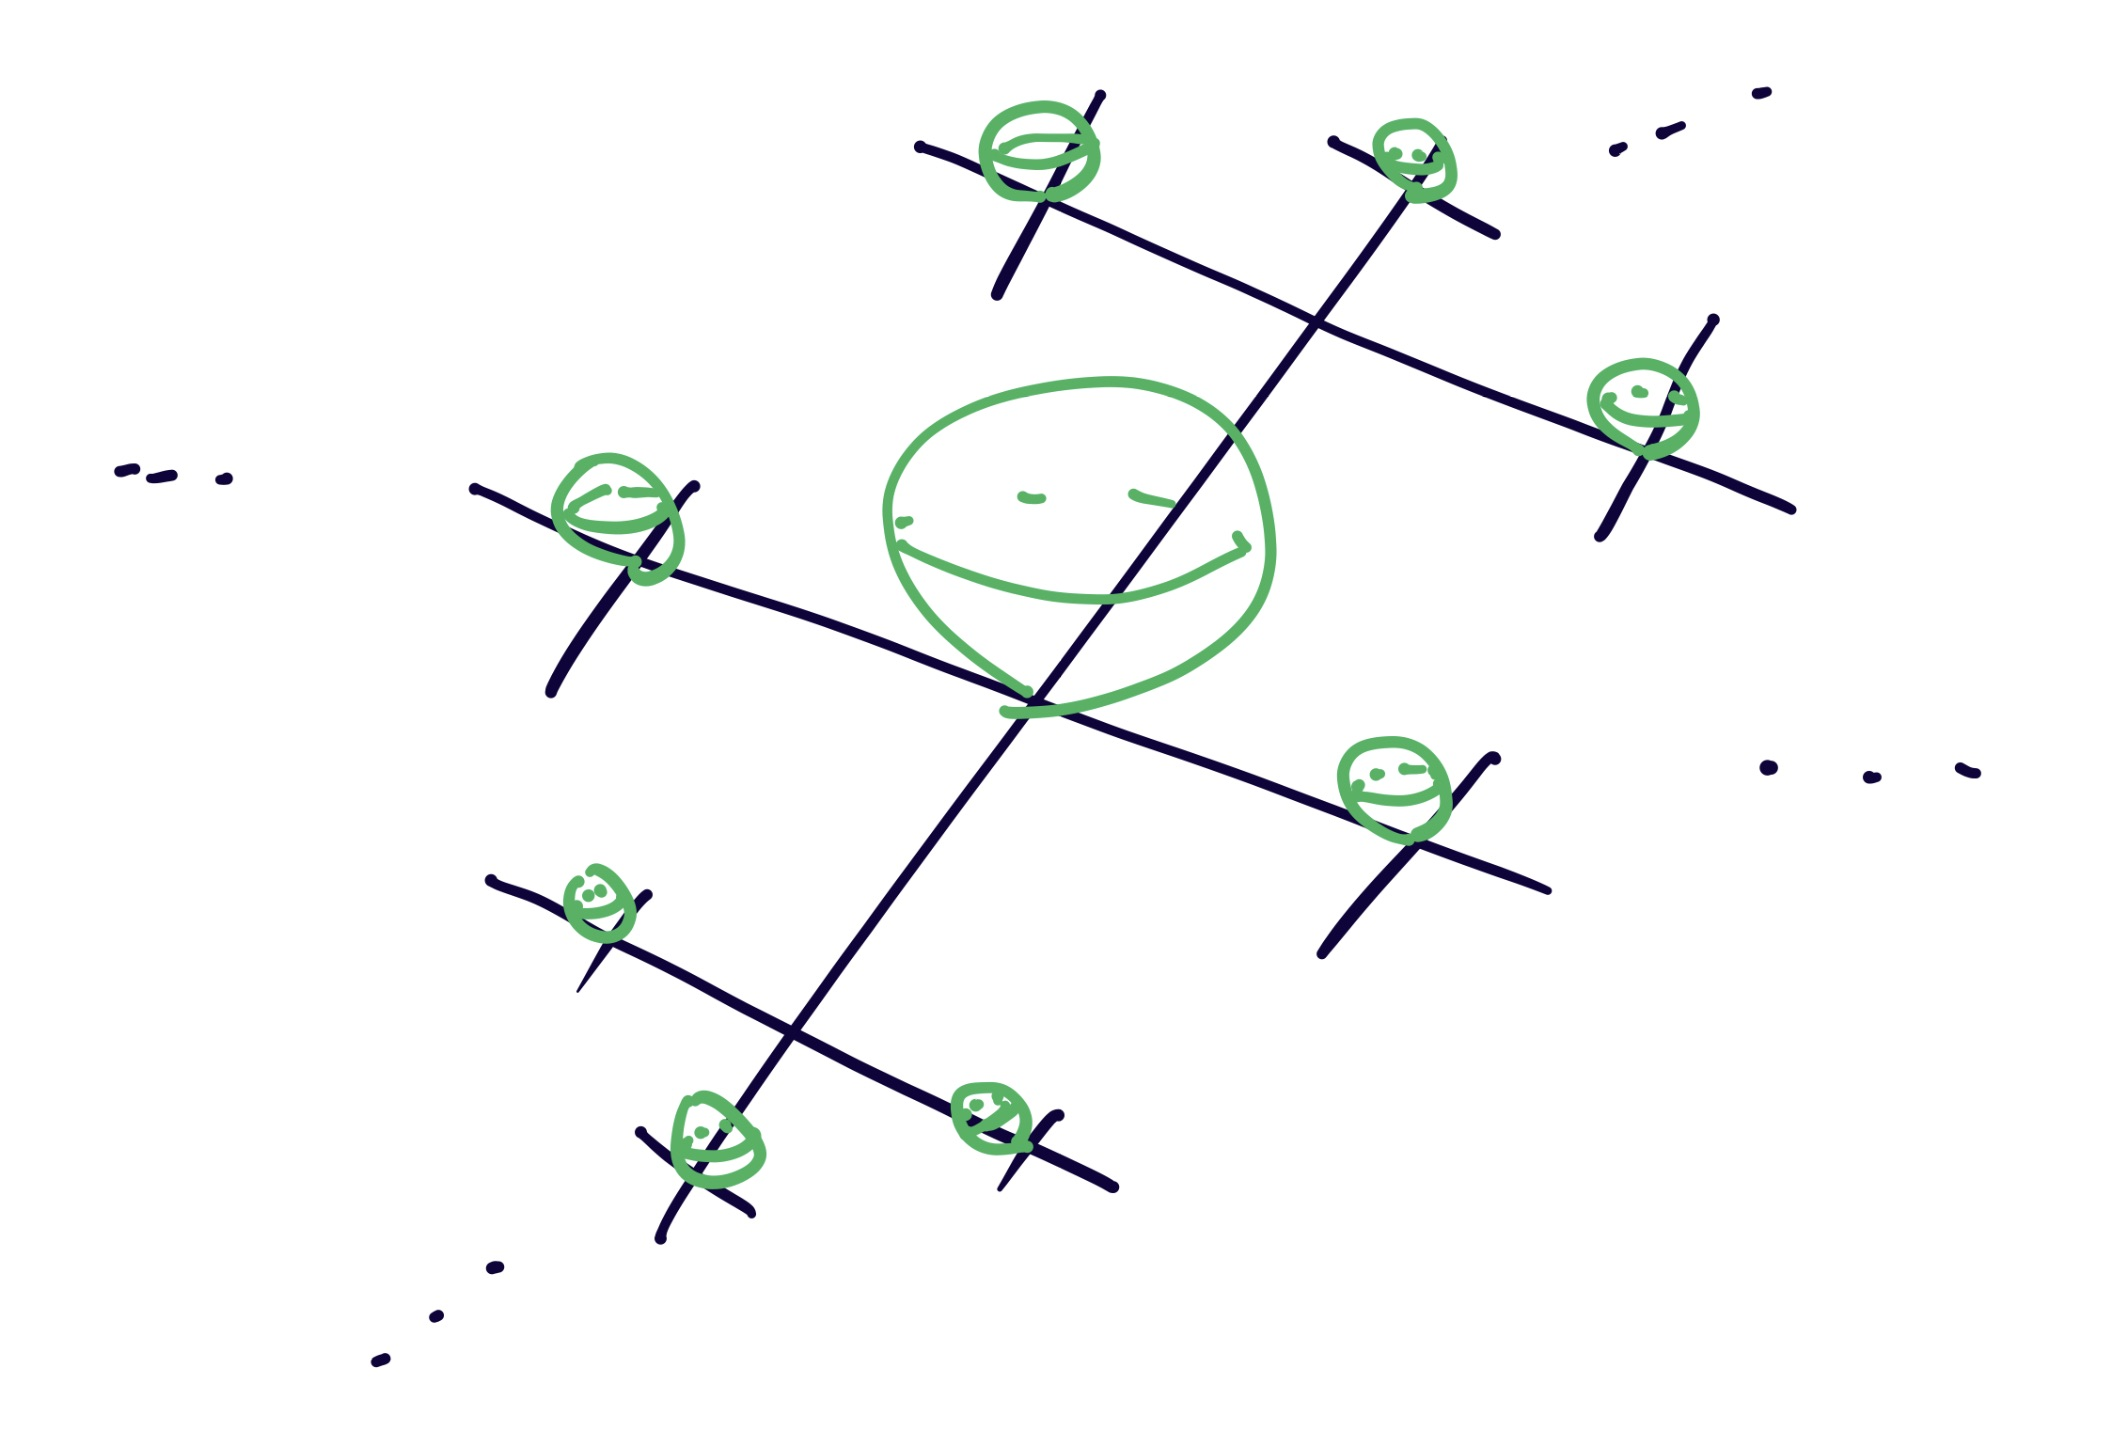
\includegraphics[width=12cm]{figures/hwk9-fig3.png}
      \captionof{figure}{Portion of the universal cover of $S^1\vee S^1\vee S^2$}
      \label{fig:prob4-1}
    \end{center}
    Contracting along the line segments between the spheres doesn't affect the homology groups and produces a countable union of spheres. This certainly doesn't have trivial homology, as once can see by Corollary 2.25 again for instance.
  \end{prf}
  \prob[\textsc{Exercise }Exercise 2.2.28]$ $
  \begin{enumerate}[(a)]
    \item Use the Meyer-Vietoris sequence to compute the homology groups of the space obtained from a torus $S^1\times S^1$ by attaching a M\"obius band via a homeomorphism from the boundary circle of the M\"obius band to the circle $S^1\times \{x_0\}$ in the torus.
    \item Do the same for the space obtained by attaching a M\"obius band to $\bRP^2$ via a homeomorphism from the boundary circle to the standard $\bRP^1 \subset \bRP^2$.
  \end{enumerate}
  \begin{prf}$ $

    \noindent \textbf{\emph{(a)}}\hspace{1em} Let $X$ be the space in question, a torus $T^2 = S^1\times S^1$ with a M\"obius band $M$ glued to $S^1\times \{x_0\}$ via its boundary. Let $U = S^1 \times (x_0 - \epsilon, x_0 + \epsilon)$ be a tubular neighborhood of $S^1\times x_0$ and let $V$ be a similar tubular neighborhood of $\partial M$. Set $A = M \cup U$ and $B = T^2 \cup V$, where $T^2$ and $M$ have been identified with their images in $X$. By construction, $U$ deformation retracts onto $S^1 \times \{x_0\} = \partial M$ and $V$ deformation retracts onto $\partial M = S^1\times \{x_0\}$, so $A$ deformation retracts to $M$ and $B$ deformation retracts to $T^2$ via the same maps composed with the identity on $M$ and $T^2$ respectively.

    By definition, $A$ and $B$ are both open, $A \cup B = X$ and $A\cap B$ is an open neighborhood of $S^1\times \{x_0\} = \partial M$ which deformation retracts onto $S^1\times \{x_0\} = \partial M$. Applying the Meyer-Vietoris sequence therefore gives us
    \begin{align*}
      ... \to \tilH_2(&A\cap B) \to\tilH_2(A) \oplus \tilH_2(B) \to \tilH_2(X) \to \tilH_1(A\cap B) \to ... \\
        &...\to \tilH_1(A)\oplus \tilH_1(B) \to \tilH_1(X) \to \tilH_0(A\cap B) \to ...
    \end{align*}
    so after applying our knowledge of these groups, we get
    \begin{align*}
      ... \to 0 \to \bZ \to \tilH_2(X) \to \bZ\to  \bZ\oplus \bZ^{\oplus 2} \to \tilH_1(X) \to 0 \to ...
    \end{align*}
    The main part of this sequence demanding close inspection is the $n = 1$ portion. The map $\Phi:\tilH_1(A\cap B) \to H_1(A) \oplus H_1(B)$ is induced by the inclusion of $A\cap B$ into $A$ and $B$. As discussed above, we have $A\cap B \simeq \partial M = S^1\times \{x_0\}$, $A \simeq M$ and $B \simeq T^2$, so instead we may think of $\Phi$ as a map $\tilH_1(\partial M) \to \tilH_1(M)\oplus \tilH_1(T^2)$ induced by the inclusions $S^1\times \{x_0\}\hookrightarrow T^2$ and $\partial M \hookrightarrow M$.

    Let $b_1$  and $b_2$ be the generators for $\tilH_1(B) = \tilH_1(T^2)$ representing the circle $S^1\times \{x_0\}$ and $\{\text{pt}\}\times S^1$ respectively, $a$ the sole generator for $\tilH_1(A) = \tilH_1(M)$ represented by the central circle of $M$, and $c$ the sole generator for $\tilH_1(\partial M)$. The circle given by $\partial M$ wraps around the central circle of $M$ twice, so the inclusion of $\partial M$ into $M$ induces a map sending $c$ to $2a$ on the level of homology. However, $\partial M = S^1\times \{x_0\}$ \emph{is} a generator $b_1$ in $B \simeq T^2$, so the inclusion of $S^1\times \{x_0\}$ into $T^2$ induces a map $c \mapsto b_1$ on the level of homology. Together, this means $\Phi(c) = 2a - b_1$, where we pick up a negative sign in the second summand due to the quirks of the Meyer-Vietoris sequence. Since $\tilH_1(A\cap B) \cong \bZ$, this fully determines the map $\Phi$, meaning $\img \Phi \cong \bZ(2a - b_1)$. Combining this with the exactness of the above sequence, we get that
    \begin{align*}
      \tilH_1(X) \cong \tilH_1(A) \oplus \tilH_1(B)/\img \Phi \cong \bZ^{\oplus 3}/\bZ(2a - b_1) \cong \bZ\oplus \bZ.
    \end{align*}
    Our analysis of $\Phi$ is also invaluable for computing $\tilH_2(X)$: since $\Phi$ took the sole generator of $\bZ$ to a nonzero element of another free group, it is injective and hence has trivial kernel. This means the map $\beta:\tilH_2(X)\to \bZ$ is trivial. The exactness of $0 \to \bZ \xrightarrow{\alpha}\tilH_2(X)$ tells us that $\alpha$ is injective, and an additional application of exactness yields $\bZ \cong \img \alpha = \ker \beta = \tilH_2(X)$.

    Because $X$ is path-connected, we know $\tilH_0(X) = 0$. For $n \geq 3$, Meyer-Vietoris tells us
    \begin{align*}
      ... \to \tilH_n(A) \oplus \tilH_n(B) \to \tilH_n(X) \to \tilH_{n-1}(A\cap B) \to ...
    \end{align*}
    which reduces to $0 \to \tilH_n(X) \to 0\implies \tilH_n(X) \cong 0$, since $\tilH_{n-1}(A\cap B)$, $\tilH_n(A)$ and $\tilH_n(B)$ are all trivial for $n \geq 3$. In summary,
    \begin{align*}
      \tilH_n(X) = 
      \begin{cases}
        \bZ \oplus \bZ & n = 1 \\
        \bZ & n = 2 \\
        0 & \text{else}
      \end{cases}.
    \end{align*}
    \bigskip

    \noindent \textbf{\emph{(b)}}\hspace{1em} First note that $\bRP^1 \simeq S^1$. One can see this by recalling $\bRP^1$ is obtained from $S^1$ by identifying antipodal points. Traversing $S^1$, we do not encounter a previously traversed point until we have moved $\pi$-radians, at which point we have returned to the chosen basepoint of $S^1$.

    Let $X$ be the space in question. We define tubular neighborhoods of $\partial M = \bRP^1$ in a similar way as above: take $U$ to be a neighborhood of $\bRP^1$ in $\bRP^2$ which deformation retracts onto $\bRP^1$ and let $V\subseteq M$ be as in part (a). Defining $A = M\cup U\subseteq X$ and $B = \bRP^2 \cup V$ means that
    \begin{itemize}
      \item $A$ and $B$ are open,
      \item $A\cup B = X$ and
      \item $A\cap B$ deformation retracts onto $\partial M = \bRP^1$ in $X$.
    \end{itemize}
    Since $\bRP^1$ and $M$ are both homotopic to the circle, we have
    \begin{align*}
      \tilH_n(A\cap B) \cong \tilH_n(A) = 
      \begin{cases}
        \bZ & n = 1 \\
        0 & \text{else}
      \end{cases}
    \end{align*}
    and
    \begin{align*}
      \tilH_n(B) \cong \tilH_n(\bRP^2) =
      \begin{cases}
        \bZ/2\bZ & n = 1 \\
        0 & \text{else}
      \end{cases}.
    \end{align*}
    For the same reasons as before, $\tilH_n(X) = 0$ for $n \geq 3$ and $n = 0$, so the only relevant portion of the Meyer-Vietoris sequence is
    \begin{align*}
      ... \to 0 \to \tilH_2(X) \to \overbrace{\tilH_1(A\cap B)}^{\bZ} \xrightarrow{\Phi} \overbrace{\tilH_1(A)}^{\bZ}\oplus \overbrace{\tilH_1(B)}^{\bZ/2\bZ} \to \tilH_1(X) \to 0 \to ...
    \end{align*}
    Let $a$ be the generator of $\tilH_1(A)$ (representing the central circle of $M$), $b$ the generator of $\tilH_1(B)$, and $c$ the generator of $\tilH_1(A\cap B)$. Applying a similar argument as before, we see that $c$ wraps around $a$ twice and hence
    \begin{align*}
      \Phi(c) = 2a - b.
    \end{align*}
    The exactness of the sequence tells us that $\Phi$ is injective so $\ker\Phi = 0$, and therefore $\img(\tilH_2(X) \to \tilH_1(A\cap B)) = \ker \Phi = 0$. However, exactness tells us the kernel of $\tilH_2(X)\to \tilH_1(A\cap B)$ must also be $0$, meaning $\tilH_2(X) = 0$. We therefore have a short exact sequence
    \begin{align*}
      0 \to \bZ \xrightarrow{\Phi} \to \bZ\oplus \bZ/2\bZ \to \tilH_1(X) \to 0,
    \end{align*}
    so
    \begin{align*}
      \tilH_1(X) \cong \bZ\langle a, b \rangle ~/~ \bZ\langle 2a - b, 2b \rangle \cong \langle a, b \rangle ~/~ \langle 2a - b, 4a \rangle \cong \bZ/4\bZ.
    \end{align*}
    Summarizing,
    \begin{align*}
      \tilH_n(X) \cong
      \begin{cases}
        \bZ/4\bZ & n = 1 \\
        0 & \text{otherwise}
      \end{cases}.
    \end{align*}
  \end{prf}
  \prob[\textsc{Exercise }2.2.31] Use the Mayer-Vietoris sequence to show that there are isomorphisms $\tilH_n(X\vee Y) \cong \tilH_n(X) \oplus \tilH_n(Y)$ if the basepoints of $X$ and $Y$ that are identified in $X\vee Y$ are deformation retracts of neighborhoods $U\subseteq X$ and $V\subseteq Y$.
  \begin{prf}
    This is a straightforward application of Mayer-Vietoris. Let $x_0 \in X$ and $y_0 \in Y$ be the basepoints identified in the wedge sum $X\vee Y$, and let $U\subseteq X$ and $V\subseteq Y$ be open neighborhoods of $x_0$ and $y_0$ respectively which deformation retract to $x_0$ and $y_0$. Define $A = X\cup V \subseteq X\vee Y$ and $B = U\cup Y \subseteq X\vee Y$. Then $A\cup B = X \vee Y$ and $A \cap B = U \cup V$. This latter set deformation retracts onto the basepoint of $X\vee Y$; simply deformation retract $U$ onto $x_0$ in $X$ and $V$ onto $y_0$ in $Y$. This map will be continuous on $U \cup V$ since $U\cap V = \{x_0 = y_0\}$ and each individual deformation retract leaves the basepoint fixed.

    The Mayer-Vietoris sequence then gives us
    \begin{align*}
      ... \to \tilH_n(A\cap B) \to \tilH_n(A)\oplus \tilH_n(B) \to \tilH_n(A\cup B) \to H_{n-1}(A\cap B)\to ...
    \end{align*}
    but because $A\cap B$ deformation retracts to a point and $A\cup B = X\vee Y$, we actually have
    \begin{align*}
      ... \to 0 \to \tilH_n(A)\oplus \tilH_n(B) \to \tilH_n(A\cup B)\to 0 \to ...
    \end{align*}
    for each $n$. The exactness of the Mayer-Vietoris sequence then implies that this map is an isomorphism.
  \end{prf}
  \prob[\textsc{Exercise }2.2.36] Show that $H_i(X\times S^n)\cong H_i(X)\oplus H_{i-n}(X)$ for all $i$ and $n,$ where $H_i = 0$ for $i < 0$ by definition. Namely, show that $H_i(X\times S^n)\cong H_i(X) \oplus H_i(X\times S^n, X\times \{x_0\})$ and $H_i(X\times S^n, X\times \{x_0\}) \cong H_{i-1}(X\times S^{n-1},X\times \{x_0\})$.
  \begin{prf}
    Given the suggestion in the problem statement, we split up this proof into lemmas.
    \begin{lem}\label{lem:problem2.2.36a}
      $H_i(X\times S^n)\cong H_i(X) \oplus H_i(X\times S^n,X\times \{x_0\})$.
    \end{lem}
    \begin{proof}
      First note that $X\times \{x_0\}$ is a retraction of $X\times S^n$ via the map $r = \id_X\times \pi_{x_0}$ which sends $X$ to itself and all of $S^n$ to $x_0$. By problem 2.1.11 (from the last homework) this means the inclusion $\iota:X\times \{x_0\}\to X\times S^n$ induces an inclusion $\iota_*:H_i(X\times \{x_0\}) \to H_i(X\times S^n)$ on homology. With this in mind, consider the long exact sequence on relative homology:
      \begin{align*}
        ...\to H_{i+1}(B,A) \xrightarrow{\partial} H_i(A) \xrightarrow{\iota_*} H_i(B) \xrightarrow{j_*} H_i(B,A) \xrightarrow{\partial} H_{i-1}(A) \xrightarrow{\iota_*} ...
      \end{align*}
      where we have written $B = X\times S^n$ and $A = X\times \{x_0\}$ to save space. By exactness and the injectivity of $\iota_*$, $\img \partial = 0$. This in turn implies $\ker\partial = H_i(B,A)$ and so $j_*$ is surjective, and hence we can insert zeros between each pair of $H_i(B,A)$ and $H_{i-1}(A)$ terms, giving us a short exact sequence
      \begin{align*}
        0 \to H_{i}(X\times \{x_0\}) \xrightarrow{\iota_*} H_i(X\times S^n) \to H_{i}(X\times S^n,X\times \{x_0\})\to 0
      \end{align*}
      for each $i$. Furthermore, because $r\circ \iota = \id$, $r_*\circ \iota_* = \id$ which means $\iota_*$ is a split map on homology. This gives us an isomorphism
      \begin{align*}
        H_i(X\times S^n) \cong H_i(X\times \{x_0\}) \oplus H_i(X\times S^n,X\times \{x_0\}),
      \end{align*}
      and because $X\times \{x_0\}\cong X$, $H_i(X\times S^n) \cong H_i(X) \oplus H_i(X\times S^n,X\times \{x_0\})$.
    \end{proof}

    Now we turn our attention to the $H_i(X\times S^n,X\times \{x_0\})$ term in the above direct sum.
    \begin{lem}\label{lem:problem2.2.36b}
      $H_i(X\times S^n,X\times \{x_0\}) \cong H_{i-1}(X\times S^{n-1}, X\times \{x_0\})$.
    \end{lem}
    \begin{proof}
      As hinted by Hatcher, this is a straightforward application of the Meyer-Vietoris sequence. The only potentially tricky part is choosing a good open cover for $X\times S^n$. Given that we've been prompted to find an isomorphism from something involving $S^n$ to something involving $S^{n-1}$, it makes sense to choose open sets $U$ and $V$ which cover $S^n$ and whose intersection deformation retracts to $S^{n-1}$. This can be accomplished by letting $U$ and $V$ be the lower and upper disks $D^n$ extending slightly past the equator of $S^n$. More explicitly, let $\epsilon > 0$ be small and set
      \begin{align*}
        U = \{(s_0,...,s_n) \in S^n ~ \mid~ s_0 < \epsilon\} \textbuff{1em}{and} V = \{(s_0,...,s_n) \in S^n ~ \mid~ s_0 > -\epsilon\}.
      \end{align*}
      \begin{center}
        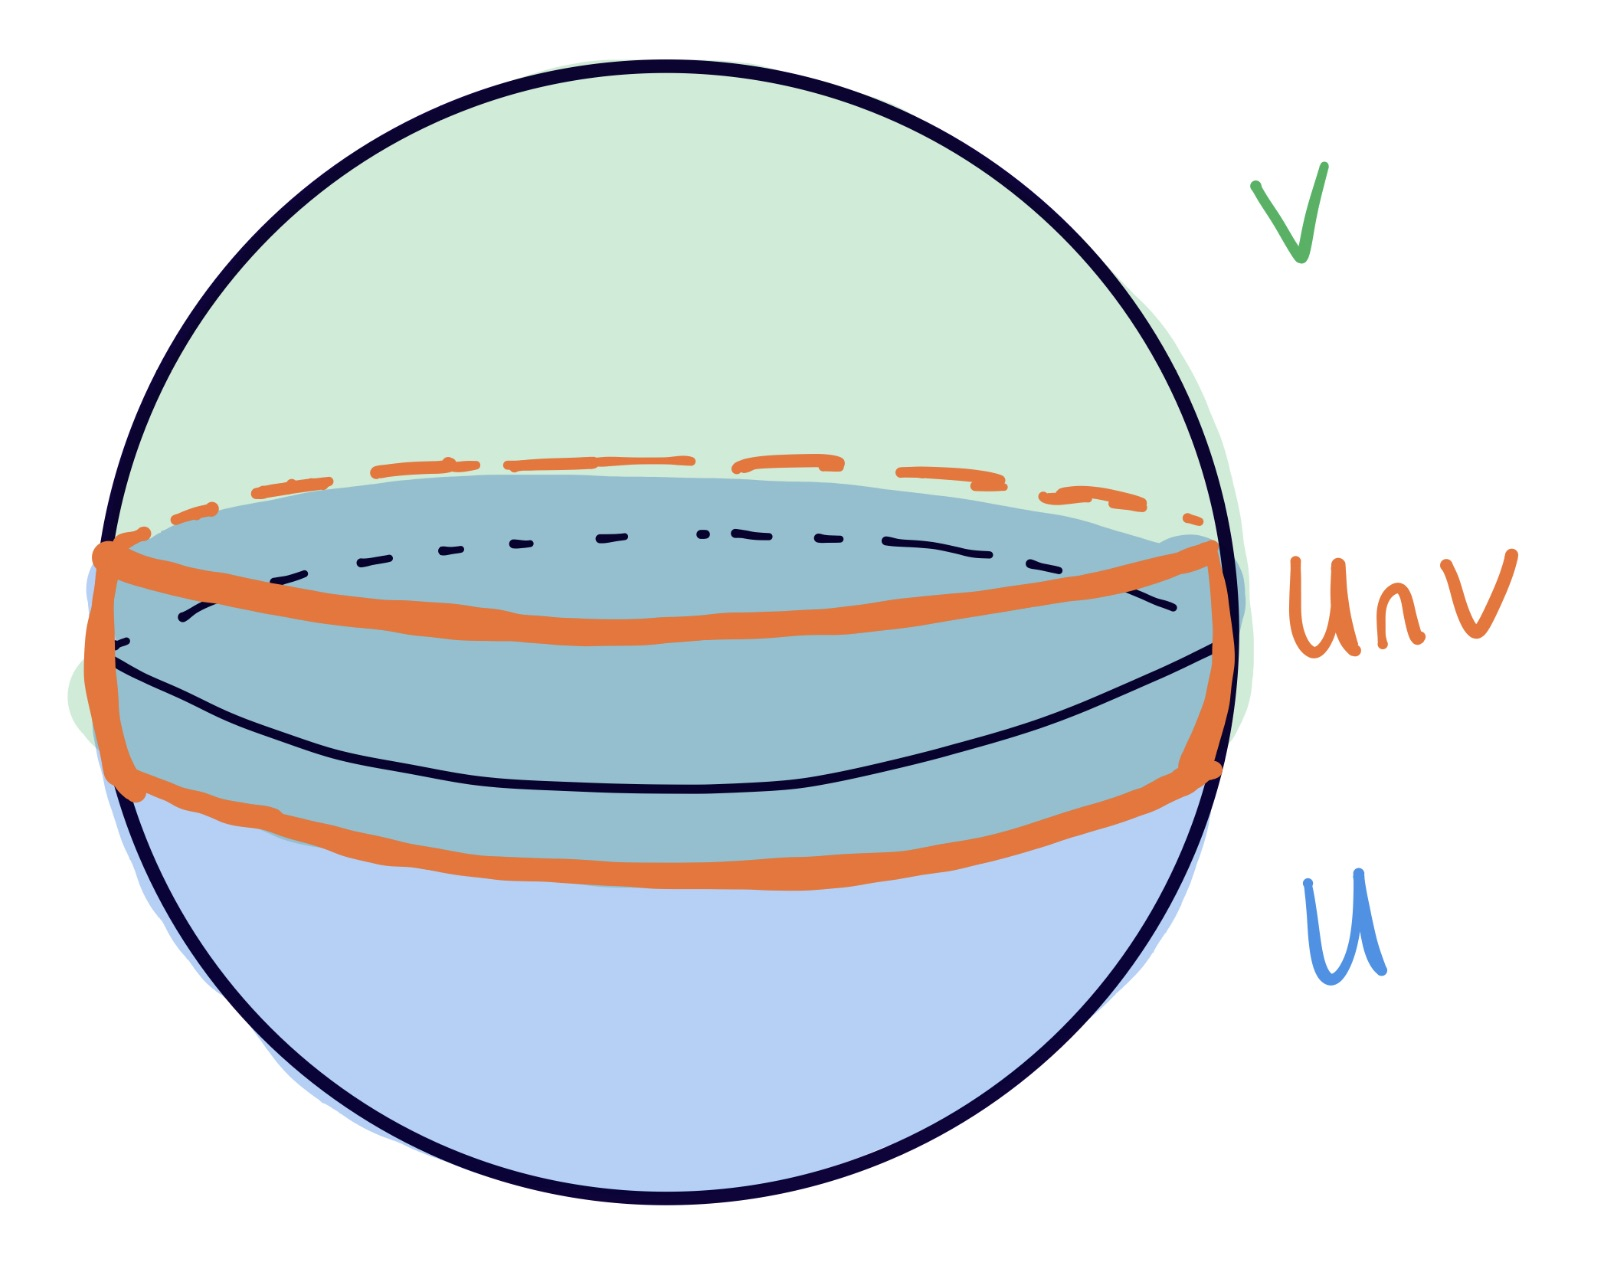
\includegraphics[width=12cm]{figures/hwk9-fig4.png}
        \captionof{figure}{Good choice of open cover for $S^n$}
        \label{fig:prob7-1}
      \end{center}
      Then $U\cup V = S^n$ and $U\cap V$ deformation retracts onto $S^{n-1} = \{(0,s_1,...,s_n) \in S^n\}$. Now define $A = X\times U$ and $B = X\times V$, so that $A\cup B = X\times S^n$ and $A\cap B \simeq X\times S^{n-1}$. Applying the relative Meyer-Vietoris to this yields the long exact sequence
      \begin{align*}
        ... \to H_n(A\cap B, C) \to H_n(A,C) \oplus H_n(B,C) \to H_n(A\cup B,C) \to ...
      \end{align*}
      where $C = X\times \{x_0\}$ with $x_0$ chosen to lie on the equator of $S^n$. Because both $U$ is a copy of $D^n$ and is hence contractible, we have that
      \begin{align*}
        H_n(A,C) = H_n(X\times U, X\times \{x_0\}) \cong H_n(X\times \{x_0\}) \cong 0.
      \end{align*}
      We get something similar for $B = X\times V$. This implies that the above relative Meyer-Vietoris sequence is actually
      \begin{align*}
        ... \to 0 \to H_n(X\times S^{n}, X\times \{x_0\})\to H_{n-1}(X\times S^{n-1}, X\times \{x_0\})\to 0 \to ...
      \end{align*}
      for each $n$, which gives us the desired isomorphic by exactness.
    \end{proof}
    With these two lemmas out the way, we can quickly complete the problem. Using Lemma \ref{lem:problem2.2.36b} inductively, we get that
    \begin{align*}
      H_i(X\times S^n,X\times \{x_0\}) \cong H_{i - n}(X\times S^0,X\times \{x_0\}).
    \end{align*}
    However, $S^0$ is a set containing two points. We may assume one of these is $x_0$, and hence 
    \begin{align*}
      H_{i-n}(X\times S^0,X\times \{x_0\})\cong H_{i-n}(X\times \{x_1\})\cong H_{i-n}(X)
    \end{align*}
    since $X$ is homeomorphic to $X \times \{x_1\}$. Applying Lemma \ref{lem:problem2.2.36a}, we conclude that
    \begin{align*}
      H_i(X\times S^n) \cong H_i(X) \oplus H_i(X\times S^n,X\times \{x_0\}) \cong H_i(X) \oplus H_{i-n}(X).
    \end{align*}
  \end{prf}
\end{homework}
\end{document}
